\documentclass[a4paper,12pt,oneside]{article}
\usepackage[czech]{babel}
\usepackage[left=1.5cm,text={18cm, 25cm},top=2.5cm]{geometry}
\usepackage[IL2]{fontenc}
\usepackage[utf8]{inputenc}
\usepackage{svg, amsmath, amsthm, amssymb}
\usepackage{times}
\usepackage{hyperref}

\begin{document}
\begin{titlepage}
  \begin{center}
	
\includegraphics[origin=c,scale=0.5]{fit}
	\\[6cm]
    {\Huge Databázové systémy}\\[5mm]
    {\LARGE Dokumentácia k projektu}\\
    \vspace{\stretch{0.618}}
    \begin{flushleft}
      \Large{Alexandra Slezáková (xsleza20)\\Matej Soroka (xsorok02)}
    \end{flushleft}
  \end{center}
\end{titlepage}

\tableofcontents
\newpage

\section{Trigger}

\subsection{map\_scale}
Trigger spustený pred vkladaním alebo upravovaní riadkov tabuľky \texttt{MAP}.\\
Kontroluje správny formát mierky mapy v stĺpci \texttt{scale} pomocou regulérneho výrazu: \texttt{(\textbackslash d)+:(\textbackslash d)+}

\subsection{Player\_PK}
Trigger spustený pred vkladaním riadka do tabuľky \texttt{PLAYER} v prípade, že nie je zadaná hodnota stĺpca \texttt{player\_id} obsahujúca primárny kľúč tabuľky.
Spolu s triggrom je vytvorená aj sekvencia, ktora zaručuje unikátnosť vygenerovaného primárneho kľúča.

\section{Procedúry}
\subsection{wrong\_class}
Procedúra pre overenie správnosti povolaní vytvorených postáv v tabuľke \texttt{CHARACTER}. Procedúra preiteruje celú tabuľku s pomocou premennej \texttt{characters\%ROWTYPE}, ktorá v každej iterácií obsahuje iterovaný riadok z tabuľky. Pri každej iterácií porovnáva reťazec uložený v stĺpci \texttt{class}. Ak sa hodnota v stĺpci nerovná jednej zo \href{https://www.dndbeyond.com/classes}{všeobecne známych povolaní}, procedúra uživateľa vypíše sa.

\subsection{who\_is\_rich}
Procedúra pomocou agregačnej funcie \texttt{avg} vypočíta aritmetický priemer hodnoty reprezentujúcej priemerný počet zlata stĺpca \texttt{gold} v tabuľke \texttt{PLAYER}, ktorý hráč vlastní. Hodnotu uloží do premennej. Následne procecúra preiteruje tabuľku \texttt{PLAYER} a porovnáva priemernú hodnotu s hodnotou v stĺpci \texttt{gold}, v prípade že je hodnota v stĺpci vačšia ako hodnota v premennej obsahujúcej priemer, hráč sa označí ako objektívne bohatší k väčšine a vypíše.

\section{Explain plan a index}
Select nám vyhľadáva počet postáv vlastnených administrátormi, kedže administrátor je podmnožina hráča, tak jeho informácie sú uložené v tabuľke \texttt{PLAYER} s jediným rozdielom, a tým je hodnota v stĺpci \texttt{role}, kde hodnota reprezentuje rolu daného hráča. Keďže rola je reťazec, tak je vhodné z neho vytvoriť index.

\subsection{Pred zavedením indexu}
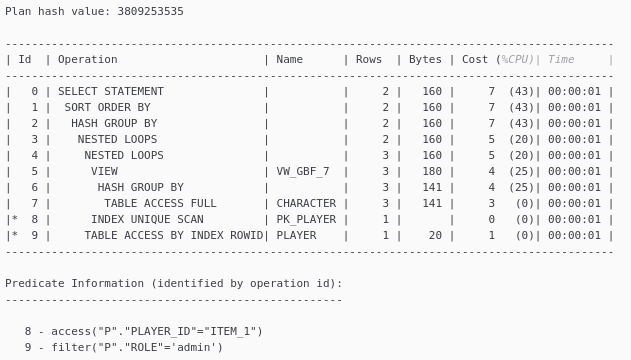
\includegraphics[origin=c,scale=0.5]{explain}\\

\subsection{Po zavedení indexu}
Pri použití indexu nám klesla výpočetná náročnost a množstvo alokovanej pamäte.\\
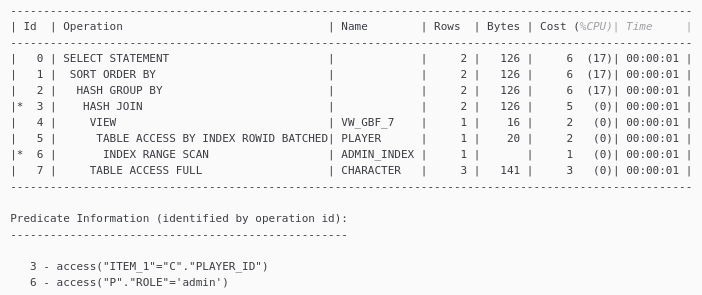
\includegraphics[origin=c,scale=0.5]{explain_second}

\end{document}
